\documentclass{article}
\usepackage[T1] {fontenc}
\usepackage[italian]{babel}
\usepackage{cite}

\usepackage{amsmath}

\usepackage{graphicx}
\graphicspath{ {./images/} }
\usepackage{float}

% Per i link nell'indice
\usepackage{hyperref}

\title{Gioco di modellamento newtoniano per il moto di un proiettile}
\author{Daniele Meloccchi, Agnese Montanaro, Matteo Savatteri}

\begin{document}
\maketitle

\tableofcontents

\section{Introduzione}
In questo documento presentiamo lo studio del moto di un
proiettile, analizzato con la tecnica dei \emph{giochi di modellamento newtoniani}
\cite{hestenes1992modeling}.

\section{Il sistema}
Il sistema che ci apprestiamo a studiare è costituito da un corpo lasciato cadare da
un piano inclinato su di una superficie, che ci permetta di individuare il 
punto esatto della caduta.  La velocità iniziale del proiettile è raggiunta e
regolata mediante il piano inclinato, sul quale il corpo in questione viene fatto scivolare
o rotolare. Questo espediente consente un maggior controllo sul momento iniziale del
proiettile. Il corpo che abbiamo studiato è una scatola di latta cosparsa di inchiostro
e la superficie tracciante è costituita da uno strato di carta (Figura \ref{fig:setup_proiettile_3}).

\begin{figure}
\centering
  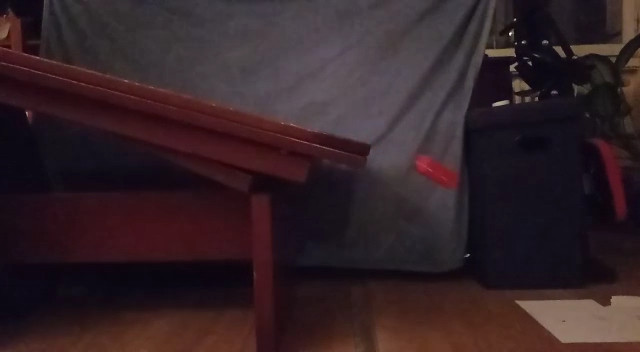
\includegraphics[width=\textwidth]{setup_proiettile_piano_inclinato_3}
  \caption{L'apparato sperimentale per studiare il moto di un proiettile.}
  \label{fig:setup_proiettile_3}
\end{figure}

\section{Gli elementi del gioco}
Il gioco di modellamento richiede prima di tutto la scelta
dei suoi componenti: tabellone e pedine.

\subsection{Il tabellone}
Il tabellone rappresenta in sistema di riferimento scelto per studiare
il sistema: nel nostro caso la coppia di assi cartesiani avente
origine nel punto in cui il proiettile si stacca dal
piano inclinato. L'asse $x$ è stato scelto parallelo al pavimento
con verso a destra e l'asse $y$ diretto come la forza gravitazionale
con verso in alto.

\subsection{Le pedine}
Le pedine rappresentano i corpi modellati come punti materiali
presenti nel sistema che stiamo studiando:

\begin{itemize}
\item La scatola di latta, di massa $m$;
\item Il pianeta Terra di massa $M \gg m$.
\end{itemize}

\subsection{Il vincolo}
Il piano inclinato nel nostro modello costituisce un vincolo,
che costringe la massa a muoversi lungo un retta:

\begin{equation}
y(x) = m x + q
\end{equation}

con $q = 0$ e $m = \tan (180 -\alpha)$, dove $\alpha$ è l'angolo
alla base del piano inclinato.
Esso può essere modellizzato come un corpo rigido privo di massa
ma dotato di inerzia infinita, che dunque risulta inamovibile.

\section{Vincere il gioco}
Per vincere il gioco, dobbiamo produrre un modello valido
der il moto del proiettile. Per valutare la validità
del modello, ci proponiamo di prevedere la velocità iniziale
del proiettile dalla conoscenza della sua altezza iniziale
$h$ e della gittata $d$ raggiunta. La velocità iniziale
così ottenuta potrà essere in seguito confrontata con quella
calcolata grazie alle specifiche del piano inclinato.

\section{Le mosse}
Possiamo compiere un certo numero di mosse, scelte tra il set
delle mosse valide, quello della dinamica newtoniana, per
condurre un gioco:

\begin{itemize}
\item Assegnare alle particelle posizioni e velocità iniziali nel sistema di riferimento scelto;
\item o interazioni consistenti con le leggi di interazione generali;
\item calcolare le traiettorie dalle leggi generali della dinamica;
\item validare il modello confrontandolo con il mondo fisico.
\end{itemize}

Tutte le precedenti sono mosse valide.

\subsection{Posizioni e velocità iniziali}
Assegnamo alla pedina $m$ la posizione iniziale $(x,y) = (-l_1,l_2)$ nel nostro
sistema di riferimento.
$l_1$ è la lunghezza del cateto maggiore del nostro piano inclinato e $l_2$
quella del cateto minore.
Per quanto riguarda le coordinate della
Terra, non ci interessa assegnarle con precisione: ci basta sapere
che $x_M = 0$ e $y_M \ll 1$.

Assegnamo al proiettile la velocità iniziale $(0,0)$, poichè essa è ferma
all'inizio del nostro esperimento, e alla Terra $(0,0)$, infatti
nel sistema di riferimento scelto è coomobile con il nostro pianeta.

\subsection{Le interazioni}
Le masse del nostro sistema interagiscono tramite una coppia di forze dirette
come la loro congiungente, di verso opposto e di valore assoluto:

\begin{equation}
|\vec{F}| = \frac{G M m}{R^2}
\end{equation}

dove $G$ è la costante di gravitazione universale e $R$ è la distanza tra i due
corpi. Siccome il moto del proiettile è ristretto ad uno spazio
molto piccolo rispetto al raggio del pianeta, possiamo assumere:

\begin{equation}
R = R_0 \approx \mbox{cost}
\end{equation}

Osserviamo che:

\begin{equation}
|\vec{a_M}| = \frac{Gm}{R_0^2} << 1
\end{equation}

dunque possiamo assumere che la presenza del proiettile non influenzi in alcun
modo il moto della Terra.

Per il proiettile invece si ha:

\begin{equation}
|\vec{a_m}| = \frac{GM}{R_0^2} = g = \mbox{cost}
\end{equation}

Da queste considerazioni possiamo dedurre che nel nostro modello
la massa $m$ è sottoposta ad una accelerazione costante
diretta verso il centro del pianeta, cioè diretta come l'asse $y$,
ma di verso opposto.

In principio il moto è vincolato dalla presenza del piano inclinato:
esso esercita sul proiettile una forza perdendicolare al piano stesso
- se si decide di trascurare l'attrito -, proporzionale alla forza di
gravità, e con componente verticale di verso opposto a quello
dell'accelerazione gravitazionale. A causa del terzo principio della
dinamica, la pedina di massa $m$ esercita sul piano una forza uguale in
valore assoluto e direzione, ma di verso opposto. Essendo il vincolo
per definizione inamovibile, la forza a cui esso è sottoposto non genera
moto.

Il proiettile nel complesso è sottoposto ad una forza risultante, somma
della forza di gravità e della forza vincolare: 

\begin{equation}
|\vec{F}_\text{piano}| = |m\vec{g} + \vec{N}| = |m(g_\perp\hat{e}_\perp + g_\parallel\hat{e}_\parallel) + N\hat{e}_\perp|   
\end{equation}

dove $\vec{N}$ è la forza vincolare e $\hat{e}_\perp$, $\hat{e}_\parallel$
sono i versori rispettivamente parallelo e perpendicolre alla direzione del
piano inclinato.

Siccome deve essere:

\begin{equation}
mg_\perp\hat{e}_\perp + N\hat{e}_\perp = 0
\end{equation}

poiché la massa $m$ non sprofonda nel piano, allora si ha:

\begin{equation}
|\vec{F}_\text{piano}| =  |mg_\parallel\hat{e}_\parallel| = mg \sin\alpha
\end{equation}

una forza costante con la stessa direzione del piano inclinato,
con componente verticale diretta verso il basso.

\subsection{Le equazioni del moto}
Da quanto abbiamo appreso sopra, sappiamo che la Terra rimane ferma
e le sue coordinate rimangono quelle iniziali per tutto il tempo
dell'esperimento.
Dall'espressione dell'accelerazione a cui è sottoposto il proiettile
quando si stacca dal piano inclinato e dalle condizioni iniziali,
possiamo invece ricavare le sue equazioni del moto parabolico:

\begin{align}
a_x(t) &= 0 \Rightarrow v_x(t) = v_{x,0} \Rightarrow x(t) = v_{x,0}t \\
a_y(t) &= -g \Rightarrow v_y(t) = - g t \Rightarrow y(t) + v_{y,0} = - \frac{1}{2} g t^2 + v_{y,0} t  
\end{align}

Misurando la gittata del proiettile $G$ e utilizzando le equazioni del
moto è possibile ricavare le velocità iniziali incognite:

\begin{align}
v_{x,0} = \sqrt{\frac{gG^2}{2(h - G\tan \alpha)}} 
\end{align}

Queste posono essere  confrontate con quelle ottenute dalla dinamica del piano inclinato.

Ricaviamo le leggi orarie della velocità lungo il piano inclinato nel sistema di riferimento
avente origine nel punto in cui si trova il proiettile quando inizia la la sua corsa, asse delle
ascisse parallelo al piano e orientato dalla sommità verso la punta, e asse dello ordinate uscente
dal piano inclinato:

\begin{align}
a_\parallel(t) &= g \sin\alpha \Rightarrow v_\parallel(t) = g \sin(\alpha) t \Rightarrow s_\parallel(t) = \frac{1}{2} g \sin(\alpha) t^2 \\
a_\perp(t) &= 0 \Rightarrow v_\perp(t) = 0 \Rightarrow s_\perp(t) = 0
\end{align}

Dalla lunghezza del piano inclinato $l$ possiamo ottenere il tempo che il proiettile
impiega per raggiungere la fine del piano, grazie alla legge oraria:

\begin{equation}
\Delta t = \sqrt{\frac{2l}{g\sin{\alpha}}}
\end{equation}

Dunque abbiamo:

\begin{equation}
v_{\parallel,0} = \sqrt{2lg\sin{\alpha}} = \sqrt{2gl_2}
\end{equation}

Applicando la trasformazione tra il sistema di riferimento del piano inclinato
e quello del tabellone:

\begin{align}
v_{x,0} &= v_\parallel\cos\alpha = \sqrt{2gl_2} \cos\alpha \\
v_{y,0} &= -v_\parallel\sin\alpha = -\sqrt{2gl_2} \sin\alpha 
\end{align}

\section{Attrito}
Possiamo tenere conto dell'attrito (dinamico o volvente) esercitato tra il piano inclinato e il punto
materiale, misurando il tempo che quest'ultimo impiega per giungere alla base del piano e ricavando
il coefficiente d'attrito dalle equazioni del moto:

\begin{equation}
\frac{1}{2} g (\sin\alpha - \mu\cos\alpha) \Delta t^2 = l \Rightarrow \mu = \tan\alpha - \frac{2l}{g\Delta t^2 \cos\alpha} 
\end{equation}

e ripetendo i conti precedenti:

\begin{align}
v_{x,0} &= \sqrt{2lg (\sin{\alpha} - \mu \cos\alpha)} \cos\alpha \\
v_{y,0} &= \sqrt{2lg (\sin{\alpha} - \mu \cos\alpha)} \sin\alpha
\end{align}

\bibliography{bibliografia}{}
\bibliographystyle{plain}

\end{document}
